\documentclass{article}\usepackage[]{graphicx}\usepackage[]{color}
%% maxwidth is the original width if it is less than linewidth
%% otherwise use linewidth (to make sure the graphics do not exceed the margin)
\makeatletter
\def\maxwidth{ %
  \ifdim\Gin@nat@width>\linewidth
    \linewidth
  \else
    \Gin@nat@width
  \fi
}
\makeatother

\definecolor{fgcolor}{rgb}{0.345, 0.345, 0.345}
\newcommand{\hlnum}[1]{\textcolor[rgb]{0.686,0.059,0.569}{#1}}%
\newcommand{\hlstr}[1]{\textcolor[rgb]{0.192,0.494,0.8}{#1}}%
\newcommand{\hlcom}[1]{\textcolor[rgb]{0.678,0.584,0.686}{\textit{#1}}}%
\newcommand{\hlopt}[1]{\textcolor[rgb]{0,0,0}{#1}}%
\newcommand{\hlstd}[1]{\textcolor[rgb]{0.345,0.345,0.345}{#1}}%
\newcommand{\hlkwa}[1]{\textcolor[rgb]{0.161,0.373,0.58}{\textbf{#1}}}%
\newcommand{\hlkwb}[1]{\textcolor[rgb]{0.69,0.353,0.396}{#1}}%
\newcommand{\hlkwc}[1]{\textcolor[rgb]{0.333,0.667,0.333}{#1}}%
\newcommand{\hlkwd}[1]{\textcolor[rgb]{0.737,0.353,0.396}{\textbf{#1}}}%

\usepackage{framed}
\makeatletter
\newenvironment{kframe}{%
 \def\at@end@of@kframe{}%
 \ifinner\ifhmode%
  \def\at@end@of@kframe{\end{minipage}}%
  \begin{minipage}{\columnwidth}%
 \fi\fi%
 \def\FrameCommand##1{\hskip\@totalleftmargin \hskip-\fboxsep
 \colorbox{shadecolor}{##1}\hskip-\fboxsep
     % There is no \\@totalrightmargin, so:
     \hskip-\linewidth \hskip-\@totalleftmargin \hskip\columnwidth}%
 \MakeFramed {\advance\hsize-\width
   \@totalleftmargin\z@ \linewidth\hsize
   \@setminipage}}%
 {\par\unskip\endMakeFramed%
 \at@end@of@kframe}
\makeatother

\definecolor{shadecolor}{rgb}{.97, .97, .97}
\definecolor{messagecolor}{rgb}{0, 0, 0}
\definecolor{warningcolor}{rgb}{1, 0, 1}
\definecolor{errorcolor}{rgb}{1, 0, 0}
\newenvironment{knitrout}{}{} % an empty environment to be redefined in TeX

\usepackage{alltt}
\usepackage[round]{natbib}
\usepackage[affil-it]{authblk}
\usepackage[hyphens]{url}
\IfFileExists{upquote.sty}{\usepackage{upquote}}{}
\begin{document}
\title{Exploring the effects of spatial aggregation}
\author[1]{Amelia McNamara%
\thanks{Some work completed while the author was partially funded by the Communications Design Group, SAP Labs. Contact: amcnamara@smith.edu}}
\author[2]{Aran Lunzer%
\thanks{Contact: aran@acm.org}}
\affil[1]{Smith College}
\affil[2]{Viewpoints Research Institute}
\date{May 2016}

\maketitle

\section{Introduction}
In this note, we present a tool that allows a user to manipulate the size and orientation of spatial aggregation units, in order to explore the effect of those parameters on the visual pattern presented. The tool is available at \\ \url{https://tinlizzie.org/spatial/}. 

\section{Background}
Aggregated data is notoriously hard for novices to grasp~\citep{KonHigRus2014, HanKap1992}. However, it is used in many situations, both symbolic (the mean) and visual (the histogram). 

When we began showing our LivelyR~\citep{LunMcN2014b} prototypes to statisticians and teachers, we were met with excitement about the ability to simply manipulate the bin width and bin offset of a histogram. Also popular was the `histogram cloud' feature that superimposed a set of slightly different histograms of the same data~\citep{McN2015}. Both interactions give a user the ability to easily manipulate parameters that they often would leave as defaults, and compare the results of different parameter choices. 

Given the popularity of our work about the impact of parameter choices on 1-dimensional distributions, we began thinking about a 2-dimensional analogue. The most natural case was mapmaking and spatial data. One common way to depict spatial data is a choropleth map, which divide area into polygons, colored by the value of a parameter measured or estimated in that area. Figure~\ref{choropleth} is a modern choropleth map, showing income disparities from average by county, over the United States~\citep{AisBut2015}. 

\begin{figure}[htbp]
\begin{centering}
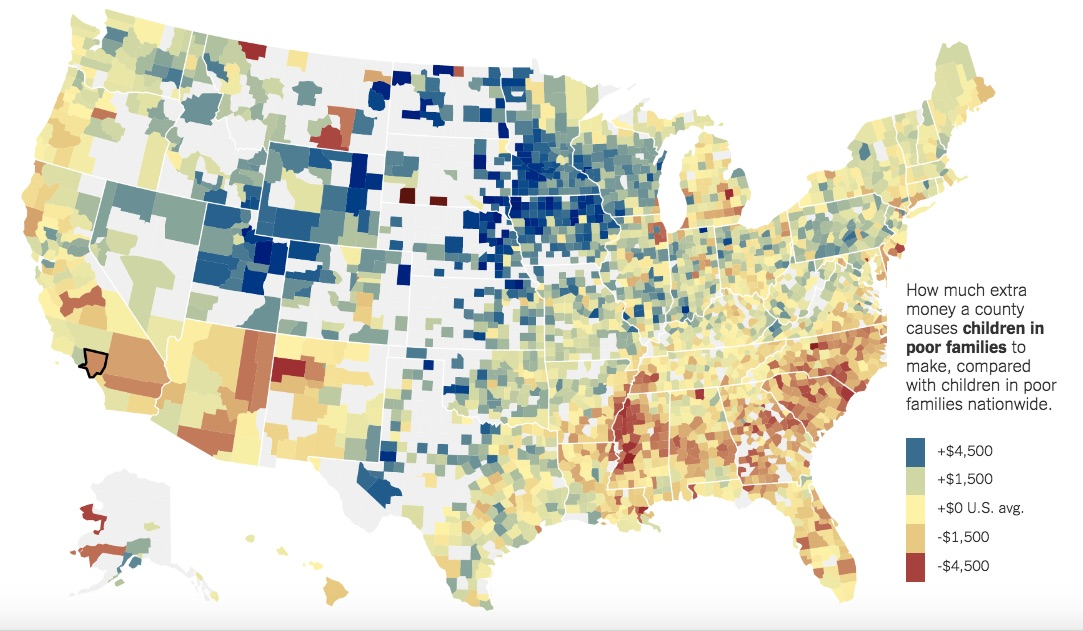
\includegraphics[width=\textwidth]{../img/choropleth}
\caption{Map of income disparities from average per county, from \cite{AisBut2015}.}\label{choropleth}
\end{centering}
\end{figure}

Many choropleth maps use polygons in the shape of political boundaries, like states, counties, and zip codes. Others use more generic polygons, like the example from 1895 shown in Figure \ref{1895} and the more modern example in Figure~\ref{wren}.

\begin{figure}[htbp]
\begin{centering}
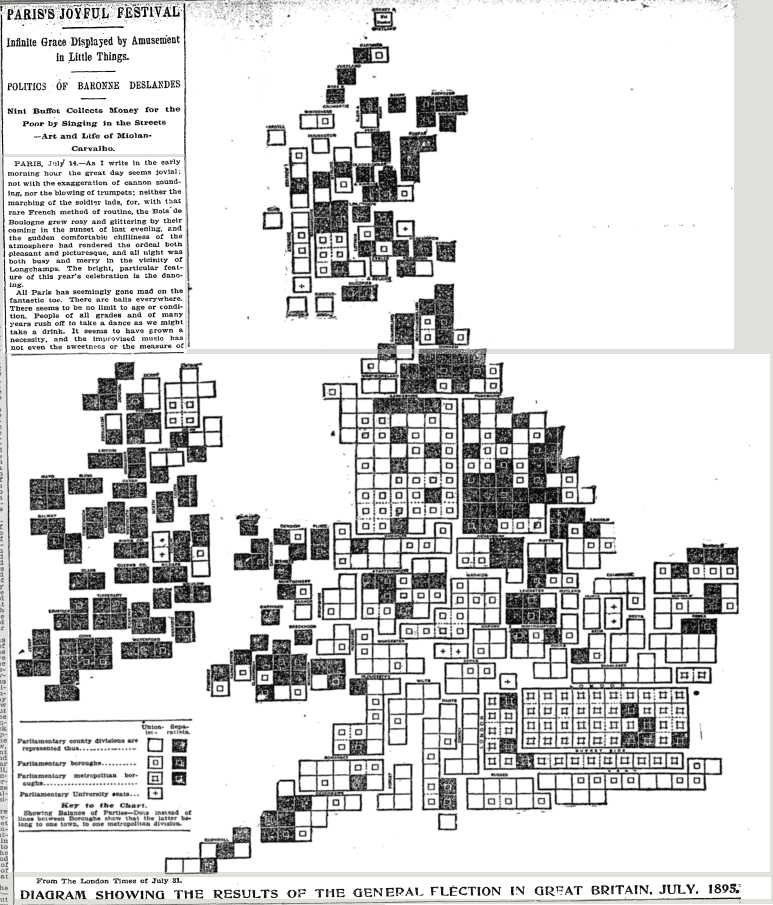
\includegraphics[height=0.4\textheight]{../img/1895}
\caption{Geometric choropleth map from 1895, from \cite{Fel2015}.}\label{1895}
\end{centering}
\end{figure}

\begin{figure}[htbp]
\begin{centering}
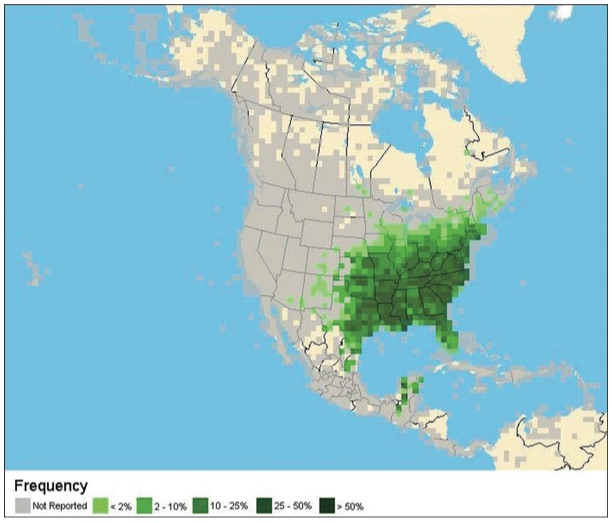
\includegraphics[height=0.4\textheight]{../img/wren}
\caption{A geometric choropleth map from 2008, showing the incidence of Carolina Wrens, binned to 100-km blocks, from \cite{SulTelWoo2008}.}\label{wren}
\end{centering}
\end{figure}


Much like the case of histograms, the visual pattern in a choropleth map is imbued with meaning by readers who forget the arbitrariness of the chosen aggregation units. 



Geographers call this phenomenon the Modifiable Areal Unit Problem (MAUP) \citep{Erv2015}. Essentially, map-making and statistical analysis is highly sensitive to the area of aggregation (e.g. Census tracts, zip codes, neighborhoods) that is used. For data that comes as points, this problem can be skirted by using the raw point data to fit models, but much spatial data is distributed in already-aggregated forms. Again, the US Census is a prime example. Because of anonymity issues, the Census Bureau can only provide data at the level of Census blocks. 

In maps where the spatial aggregation units vary in size and shape (for example, the US States), large, rural areas tend to have fewer incidences of things like homicide and cancer, which can make them appear to be ``better'' in some way than their small, densely-populated counterparts. Trying to correct for this flaw by using proportions based on population size or area adds another problem---the areas with smaller populations have higher variance, so they will appear to have higher or lower rates than average. Because of this, some statisticians argue that ``all maps of parameter estimates are misleading''~\citep{GelPri1999}. 

This work does not try to address the underlying statistical issue of generating more robust estimates from pre-aggregated data, but rather seeks to make visible the possible effects of slight variations in aggregation. 

There are two varieties of MAUP that are commonly discussed: scale MAUP and zone MAUP. The scale problem is related to the scale of the areal unit you have chosen to use. Is it large (like a state) or small (like a Census block)? The zone problem has more to do with the shape of the units. Similarly sized, but differently shaped units (imagine squares versus hexagons) can provide very different patterns. 

Notice that I am saying ``imagine" and ``like." This is because there are surprisingly few demos that actually show this phenomenon in action. Sometimes, information about MAUP will show two or three discrete possibilities of aggregations of the same data, but usually only with toy data. The figure that is used in most explanations is shown in Figure~\ref{MAUP}~\citep{Pen2014, Erv2015}. 

\begin{figure}[htbp]
\begin{centering}
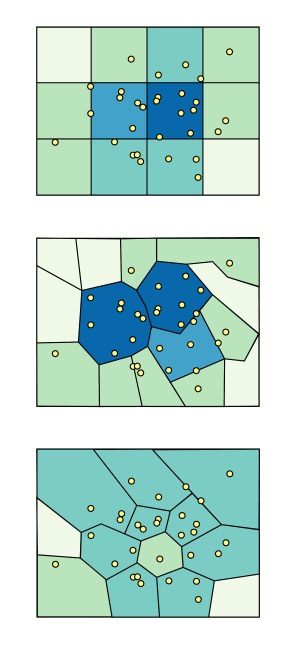
\includegraphics[height=0.5\textheight]{../img/MAUPZone1}
\caption{Typical figure used to illustrate the MAUP, taken from \cite{Erv2015}.}\label{MAUP}
\end{centering}
\end{figure}

\begin{figure}[htbp]
\begin{centering}
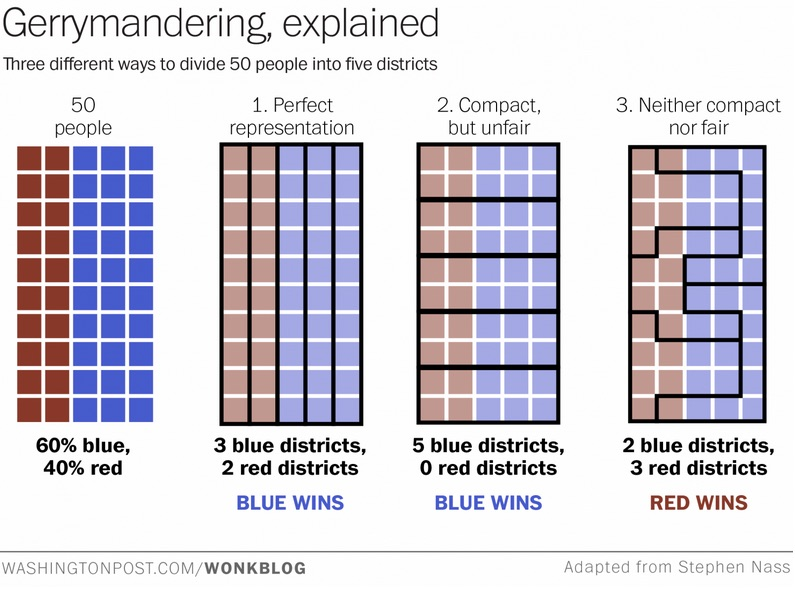
\includegraphics[width=0.8\textwidth]{../img/gerrymandering}
\caption{``The best explanation of gerrymandering you will ever see,'' from \cite{Ing2015}.}\label{gerrymandering}
\end{centering}
\end{figure}


The most publicized examples of the MAUP tend to be related to political gerrymandering of electoral boundaries. Depending on how districts are drawn, election results can be swung wildly in favor of one candidate or another. However, even in the case of gerrymandering, theoretical language like ``Suppose there's a state that [...]'' is often used, rather than concrete interactives~\citep{Coh2015}. Even in pieces that use visuals, toy examples are king, as seen in Figure~\ref{gerrymandering}~\citep{Ing2015}.


Gerrymandering is a more complex version of the MAUP, because there is more at stake than simply the location of voters. Even people in the same political party can have very different ideas about how districts should be drawn---should they contain many like-minded people, or those with similar demographics? Or should they seek to be diverse in every sense of the word? Should they follow geographic boundaries or strive for geometric compactness? 

Again, we are not trying to solve this problem. Rather, we aim to present a tool that allows users to see the effects of various spatial aggregation levels.


\section{The tool}

The tool, as it stands, is an HTML page using javascript (including d3.js and leaflet.js) to provide interaction. An OpenStreetMaps map is used as the base, and spatial point data is layered on top. Then, regular polygon aggregation units are provided, and colored according to the number of points they contain. A screenshot is shown in Figure~\ref{tool}.

\begin{figure}[htbp]
\begin{centering}
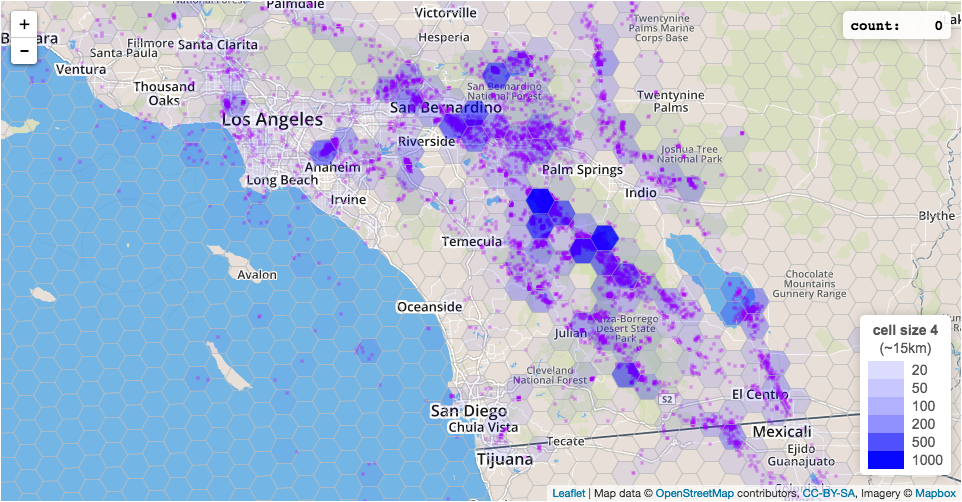
\includegraphics[width=\textwidth]{../img/tool.png}
\caption{California earthquakes from 2014, binned using hexagons.}\label{tool}
\end{centering}
\end{figure}

It supports either squares or hexagons as the polygon aggregation units, and provides 8 possible sizes, which can be moved between smoothly. 

The polygons can be scaled, moved, and rotated. The base map can also be zoomed and moved, although the interface does not support base map rotation. 

Interaction controls, as they stand now:
\begin{itemize}
\item \textbf{s} and \textbf{h} toggle the \textbf{s}quares and \textbf{h}exagons, respectively
\item The \textbf{space bar} turns the data on and off, and fades out the base map
\item \textbf{drag} moves the map, and the polygons along with it
\item \textbf{Shift} + \textbf{drag} moves the polygons without moving the map
\item \textbf{scroll wheel} or zoom buttons zoom the map, maintaining the size of polygon binning unless a threshold is breached. (The system only supports a certain number of polygons on a single screen, so if a user is zoomed in with small polygons and then zooms out, the interface will eventually change the relative size of the polygons)
\item \textbf{Shift} + \textbf{scroll wheel} zooms the size of the polygons in or out
\item \textbf{option} + \textbf{scroll} (side to side) rotates the polygons. 
\end{itemize}

\section{Use of the tool}
The tool was demoed at OpenVisConf in McNamara's talk, ``Do you know Nothing when you see it?``~\citep{McN2016f}. 


\section{Further work}

The tool as it stands is already a fun thing to play with. As you move bins around, you can watch the spatial pattern shift (or not). It provides a clear improvement on static maps using similar spatial aggregation~\citep{SulTelWoo2008, Fel2015}. We have observed that it is just as interesting to watch someone else manipulate the interface, because you can separate yourself from the immediacy of the interaction. 

However, we are already thinking of many extensions. Most important will be a way to compare some number of maps of the same data, with different aggregations. One thought is just to display a trailing history of the last 12 views, but there could be a way to ``lock'' one view into the list for comparisons. 

Past that, a few particularly salient examples of spatial patterns that show large variation in spatial pattern will help motivate the usefulness of the tool. We encountered a catch-22 when building this tool. It was hard to think of an example that would show large variation without the tool to visualize it, and it was hard to build the tool without a motivating example. Once some illustrative cases have been identified, we hope to publish an interactive essay for a broad audience. 

In the context of gerrymandering, it would be great to have a more specialized interface to allow users to manipulate voting districts to see the predicted effect on election outcomes. We have thought through several approaches to this problem, and the method that currently seems most reasonable would be to display district boundaries with the Census blocks of which they are composed, and allow users to indicate blocks they want to switch in and out of districts. A more automated approach would have the interface automatically displace districts by some number of blocks in each direction, and display the most different patterns that could be produced. 

From a more statistical perspective, this platform could provide a nice way to visualize the effects of up-, down-, and side-scaling~\citep{Atk2013, Kyr2004}. It could also be combined with data augmentation to help add more detail to pre-aggregated data, as with the tool Disser~\citep{Mar2014}. 

\clearpage



 
\bibliographystyle{plainnat}
\bibliography{/Users/amelia/Dropbox/ReadingLibrary.bib}
\end{document}
